\chapter{Literature Review}

\section{Introduction}

This literature review begins with an introduction to current work on the design and classification of 
anisotropic colloidal particles, and examples of real-world systems incorporating colloidal anisotropy.
This is followed by a discussion of current techniques for the fabrication of anisotropic colloids,
the theory of their self-assembly and experimental results.  Flow lithography is then reviewed in detail
to explore different forms of anisotropy which may be targeted by this technique.  Finally we review the current
state-of-the-art in the characterization of colloidal suspensions by particle tracking in microscopy image data, and
potential extensions of this technique for tracking anisotropic particles.

\section{Anisotropic and Patchy Colloids}

\subsection{Dimensions of Anisotropy}

\begin{figure}[h]
\begin{center}
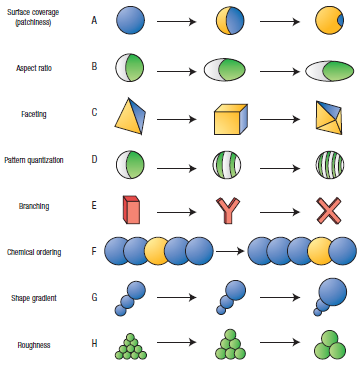
\includegraphics{figures/glotzer-anisotropy-dimensions.png}
\end{center}
\caption{Anisotropy dimensions proposed by Glotzer and Solomon~\ref{glotzer-solomon-assembly} to classify 
different forms of particle anisotropy.}
\label{fig:glotzer-dimensions}
\end{figure}

While the self-assembly of colloidal particles can produce structures with a variety of potential applications~\ref{??}, 
the range of structures which may be produced by conventional spherical colloids is limited.  One way to address this is to 
introduce colloidal particles which incorporate one or more forms of anisotropy, in which the 
particle is altered such that the interaction between two or more particles becomes non-uniform depending on 
their relative orientations.  These alterations may be based on the shape of the particles, the chemical makeup, or 
some combination of the two.

% Find many of the references in the following paragraph in Glotzer and Solomon's 2007 NatMat paper.
In a 2007 article in \textit{Nature Materials}~\ref{glotzer-solomon-assembly}, Glotzer and Solomon propose a system of anisotropy 
dimensions shown in Fig.~\ref{fig:glotzer-dimensions}. These include shape-based dimensions such as aspect 
ratio, faceting, branching, shape gradient 
and roughness (Fig.~\ref{fig:glotzer-dimensions}(B,C,E,G,H)) and dimensions based on the presence of
multiple chemistries such as surface coverage, pattern quantization and chemical ordering 
(Fig.~\ref{fig:glotzer-dimensions}(A,D,G)).  These dimensions do not necessarily 
represent an exhaustive list of the types
of anisotropy which are theoretically possible, but are an observational list of anisotropy types which have been observed in the
recent literature.  For example, rod-shaped or ellipsoidal particles of moderate aspect ratio have been fabricated 
by a wide variety of techniques including lithography~\ref{??} and particle distortion~\ref{solomon-confocal}; branched 
tetrapods have been fabricated of gold~\ref{??} and CdTe~\ref{??}; and chemically patterned particles have been produced
through microfluidic means~\ref{??} as well as by conventional photolithography~\ref{??}.  This list of dimensions may therefore
be seen as a useful framework for classification: by combining multiple dimensions, more complex types of particles may be 
developed (Fig.~\ref{fig:dimensions combined}), or a complex particle may be classified in terms of which dimensions it includes.
New forms of anisotropy may be identified as those which cannot be decomposed into dimensions already identified.

\begin{figure}[h]
\begin{center}
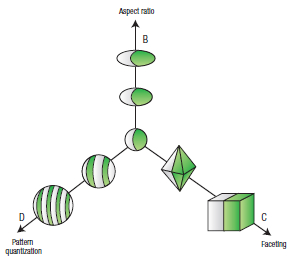
\includegraphics{figures/glotzer-combine-dimensions.png}
\end{center}
\caption{Multiple anisotropy dimensions may be combined to yield more complex types of particles.~\ref{glotzer-solomon-assembly}}
\label{fig:dimensions-combined}
\end{figure}

\begin{figure}[h]
\begin{center}
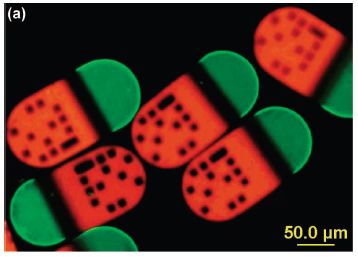
\includegraphics{figures/tan-dna-barcode.png}
\end{center}
\caption{``Barcoded'' PEG-DA particles which incorporating a DNA probe and fluorescent dyes~\ref{tan-barcode}.}
\label{fig:tan-particles}
\end{figure}

As an example of a particle which combines many types of anisotropy, 
consider the ``barcoded'' particles described in \textit{Tan et al.}~\ref{tan-barcode} for DNA analysis (Fig~\ref{fig:tan-particles}).
These particles have multiple aspect ratios (dimension B); faceting, due to the flat top and bottom surfaces (C); and pattern
quantization due to the three different chemistries included (D).  An additional form of anisotropy, the barcoding, may be seen
as a new dimension or as a more complex instance of pattern quantization.  While these particles are larger than typical colloidal
dimensions, they illustrate these principles vividly and it is reasonable to suspect they may be miniaturized.

\subsection{Theory of self-assembly}
\begin{figure}
\label{fig:glotzer-sim-assembly}
\end{figure}

\subsection{Fabrication of anisotropic colloids}

\begin{figure}
\caption{Janus spheres fabricated by emulsion technique~\ref{granick-janus}.}
\label{fig:granick-janus-spheres}
\end{figure}

\begin{figure}
\caption{PMMA rods are fabricated by (a) embedding PMMA spheres in PDMS, (b) stretching the PDMS while heated and allowing it 
it to cool, and (c) dissolving the PDMS to reveal ellipsoidal rods.}
\label{fig:solomon-rods}
\end{figure}

\begin{figure}
\label{fig:branched-particles}
\end{figure}

\begin{figure}
\label{fig:faceted-particles}
\end{figure}

\begin{figure}
\label{fig:PRINT}
\end{figure}

\begin{itemize}
\statement{Fabrication of Janus spheres: Granick, etc}
\statement{Fabrication of rods}
\statement{Fabrication of Janus rods}
\statement{Faceted particles (crystal growth etc)}
\statement{Flow lithography}
\statement{PRINT particles}
\end{itemize}


\begin{itemize}
\statement{Glotzer work on spherical patchy colloids}
\statement{Other self-assembly of spherical colloids}
\statement{Review self-assembly of non-spherical patchy colloids: focus on Janus rods}
\end{itemize}

\subsection{Experimental self-assembly}
\tempfigure{Small clusters of Janus spheres; wormlike chains; Granick}
\tempfigure{Multi-panel figure: other assembly}
\begin{itemize}
\statement{Hydrophobic/hydrophilic: Granick, clusters}
\statement{Charge-based assembly}
\statement{Magnetic assembly}
\statement{DNA-based assembly}
\end{itemize}

\section{Flow Lithography}

One technique for the fabrication of structured particles which has undergone active development in recent years is 
\textit{flow lithography}, a technique developed by Patrick Doyle at MIT which combines microfluidics with 
UV lithography.

\figone{fig:sfl-schematic}{figures/literature-review/doyle-sfl-schematic.png}{\linewidth}{
Schematic of stop-flow lithography experiment.~\cite{dendukuri-sfl}}

\figone{fig:sfl-o2-inhib}{figures/literature-review/doyle-sfl-o2-inhibition.png}{\linewidth}{
Oxygen inhibition of photopolymerization in a PDMS microfluidic device.~\cite{dendukuri-oxygen}}

In a typical continuous flow lithography experiment, we construct a microfluidic device out of polydimethylsiloxane (PDMS)
which contains a simple straight microchannel with cross-sectional dimensions between 5-400~\microns. As a feedstock
material we use some fast-photocuring low-viscosity liquid, typically a photocurable monomer solution. The device is 
placed on a microscope which includes some UV illumination source which may be reversed through the optical path (i.e.
it is emitted at the objective lens) and a fast electronic shutter. A typical example might be a conventional 
fluorescence microscope with a mercury lamp.  A photomask defining the particle geometry is placed at the microscope
field stop so that it may shape the UV beam.
To fabricate particles, the photocurable liquid is pumped through the microchannel, and the microchannel is oriented
parallel to the microscope's focal plane. The microscope objective is focused on a place inside the channel, and the
electronic shutter is opened at intervals. If the UV light is intense enough and the liquid is moving at a slow enough speed,
the UV-exposed region will cure into one or more solid particles.  
The flow of the liquid carries these particles out of the ``active 
region'', and provides fresh material.

The particle geometry is defined by a combination of the photomask and the microchannel.  The two-dimensional cross-section
is determined by the shape of the UV beam at its intersection with the microchannel, and the particle height is defined by
the height of the microchannel. The ``top'' and ``bottom'' of the particles, where they meet the upper and lower
microchannel surfaces, conform roughly to the shape of these surfaces and are generally flat.
The particles may thus be viewed as 3D extrusions of the 2D mask.  Friction or sticking with these top and bottom
surfaces are prevented in the case where PDMS is the channel material and a hydrogel monomer is the feedstock: hydrogel
curing is inhibited by the presence of oxygen, and PDMS is oxygen permeable. This results in the formation of an 
``inhibition layer'' along the internal surfaces of the channel where the liquid will not cure, preserving the mobility 
of the particles. This layer is typically about 1 \microns thick.
The resolution and quality of the 2D pattern 
is affected by the focus of the microscope (defocusing will produce blurred boundaries), the resolution of the mask,
and the magnification and numerical aperture of the objective lens.  

\subsection{Stop flow lithography}
\label{sec:SFL}

In a 2007 article in \textit{Lab On a Chip}, Dendukuri \textit{et al.} outline an innovation on flow lithography
called \textit{stop-flow lithography} (SFL).~\cite{dendukuri-sfl} In SFL, the cure-during-flow
\index{stop-flow lithography} \index{SFL}
process in conventional flow lithography is replaced with a flow-stop-cure process in which the microchannel flow
is allowed to come to a halt before UV exposure. This change allows for a substantial improvement in both 
fabrication resolution and throughput.

First, resolution is improved because stopping the microchannel flow minimizes the effect of polymerization
``smearing'', which distorts the shape of the resulting particles.
When flowing monomer solution is exposed to UV light for some finite time, any monomer which occupies the exposed volume 
during that time begins to undergo photo-polymerization.  Some of the solution will flow out of this region 
during this time, and be replaced by additional solution from up-stream. This results in a particle which is ``smeared''
or ``stretched'' along the axis of flow, and does not precisely reproduce the shape defined on the mask.  
\textbf{Work out some minimum-resolution theory here.}
When flow is 
stopped, this effect is minimized, and the only limitations imposed on the resolution are due to the optical system,
the mask resolution and materials constraints.

Second, throughput is greatly increased because higher rates of flow may be used during the periods when pressure is
applied.  In continuous-flow lithography, the rate of flow must be kept relatively slow to allow curing to take place.
Once particles have cured, no exposure step may take place until this flow has carried the particles out of the
exposure region and fresh monomer has been supplied to carry out another cure step.  In SFL, the rate of flow
may be arbitrarily high within the constraints of the device, as the cure step is carried out when the flow is stopped. 
When the cure step is finished in SFL, a high pressure is applied to quickly clear the exposure region, followed by a 
short pause to allow the fluid to stop flowing.  This procedure has allowed rates of production as high as 
$10^5$ particles min$^{-1}$.~\cite{dendukuri-sfl}

Note that the advantage in throughput is reduced somewhat when the experiment design necessitates a long pause step
after the flow. The length of this pause step is dependent on the fluid viscosity, but especially on the 
response time of the PDMS device.  When a high pressure is applied to elastic PDMS microchannel, the 
walls of the channel deform to allow it to expand.  Removing that pressure, as in SFL, produces a ``squeeze flow''
phenomenon in which the relaxation of the device walls generates some fluid flow within the channel. The cure step 
cannot take place until this flow has ceased.  In Dendukuri \textit{et al.} (2007), this phenomenon is studied in detail,
and a response time $\tau_r$ is calculated to scale as

\begin{equation}
\tau_r \sim \frac{\mu L^2 W}{EH^3}
\end{equation}

where $L$ is the channel length, $W$ is the channel width, $H$ is the channel height and $E$ is the elastic
modulus of PDMS.  Note that this response time is not dependent on the input pressure, so that relatively high
flow rates may be used without affecting the length of the pause step. However, this scaling becomes pressure-dependent
and more complicated when the deformation in channel height $\Delta h$ is comparable to $H$.~\cite{dendukuri-sfl}

\subsection{Multiple-component FL}

Polymeric particles consisting of multiple components of different chemistries may be fabricated by taking advantage
of laminar flow in microchannels.  In the laminar flow regime, several different streams may flow in parallel through
the same microchannel without turbulence, with mixing limited to that caused by diffusion.~\cite{?}  Diffusion alone
will produce very little mixing, so that a sharp boundary between two streams may spread only a few microns over
millimeters of flow.~\cite{?}  The result is a multiple-stream microchannel flow in which multiple materials
co-exist and are geometrically distinct.

If each co-flowing stream is made up of a photopolymerizable solution with similar curing kinetics, one may perform
flow lithography using a mask which illuminates several streams at once to produce particles which contain geometrically
distinct regions of different chemical makeup.  A simple case 
is demonstrated in Dendukuri \textit{et al.}~\cite{dendukuri-sfl}
for SFL, in which dyed and un-dyed PEGDA solutions are cured in the laminar flow regime to produce particles whose
fluorescence is confined to one part of the particle.  Fabrication of amphiphilic microparticles containing both
hydrophobic and hydrophilic materials is demonstrated in another Dendukuri paper in 
\textit{Langmuir}~\cite{dendukuri-amph}, and particles which incorporate biomolecule probes and lithographically-defined
``barcodes'' in different regions are fabricated by Pregibon \textit{et al.} in a 2007 paper in 
\textit{Science}.~\cite{pregibon-dna}

\section{Particle Tracking}

\tempfigure{Particle tracking illustration}
\tempfigure{Solomon rod tracking}
\tempfigure{Illustrate morphological processing}
\begin{itemize}
\statement{Crocker and Grier: IDL particle tracking}
\statement{Solomon: rod particle tracking}
\statement{Other relevant tracking?}
\statement{Basic review of morphological image processing}
\end{itemize}
